\documentclass[a4paper]{article}
\usepackage[dutch]{babel}
\usepackage{geometry}
\usepackage[utf8]{inputenc}
\usepackage{hyperref}
\usepackage{listings}
\usepackage{graphicx}
\usepackage[x11names, rgb, html]{xcolor}

% dimensions
\geometry{left=3cm, top=3cm, right=3cm, bottom=3cm}

% font
\usepackage{DejaVuSans}
\renewcommand*\familydefault{\sfdefault}
\usepackage[T1]{fontenc}

% hyperlinks
\hypersetup{%
  colorlinks=true,
  linkcolor=blue,
  urlcolor=cyan,
}

% image
\graphicspath{{img/}}

% lists
\providecommand{\tightlist}{%
\setlength{\itemsep}{0pt}\setlength{\parskip}{0pt}}

% preamble
\title{Experiments}
\author{Tim Visée \& Nathan Bakhuijzen}
\date{October 2018}

\begin{document}

  \pagenumbering{gobble}
  \maketitle
  \begin{figure}[h]
    \centering
    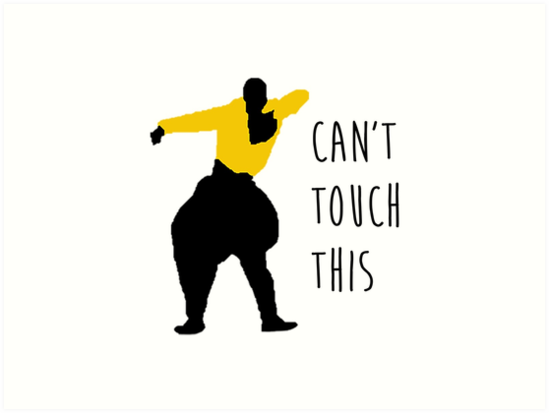
\includegraphics[width=\linewidth]{cant-touch-this}
  \end{figure}
  \clearpage

  \section{Recognized motions}
  In this document, we will list all the motions that are recognized by
  \textit{Can't Touch This}. These experiments can be conducted by first setting
  up the platform itself. Instructions for this can be found in the manual.
  After setting everything up, conducting the experiments is a piece of cake.
  Start up the platform, open a webbrowser and go to
  \href{http://localhost:8000}. Click on `Visualize' to view your fingers being
  traced.\\

  Please try to make the following gestures above the LeapMotion sensor. You
  will receive visual feedback if a gesture has been made succesfully. Try to
  succesfully complete each gesture at least 5 times for consistency sake.

  \begin{itemize}
    \tightlist
    \item Straight line
    \item Circle clockwise
    \item Circle counter-clockwise
    \item Big circle clockwise
    \item Big circle counter-clockwise
    \item Triangle clockwise
    \item Triangle counter-clockwise
    \item Mini square clockwise
    \item Square clockwise
    \item Square counter-clockwise
  \end{itemize}

  \section{Detection speed}
  Another important aspect of a gesture detection system, is the speed, or
  rather, delay for correctly detecting a performed gesture. To better define
  the term delay, we've chosen the following description: the time it takes for
  the platform to show the name of the correct gesture in the console, after a
  gesture has been completely performed above the sensor.

  \paragraph{}
  Since it can be tricky to accurately measure the time difference between the
  invocation and the action here, we've decided to use a camera to record 20
  invocations. With the resulting footage, we'll be able to count delay in
  frames, with precision accurately enough for our use case. The gesture that we
  choose was the square, as is has quite distinctive corners.

  \paragraph{}
  After performing the test it was immediately quite clear that delay varies
  greatly. The \emph{delay} varied from about 5 to 11 frames. With a speed of 60
  frames per second, each frame is about 17 milliseconds. This defines a delay
  varying between 85 to 187 milliseconds. There were two outliers with a delay
  of 16 to 22 frames which translate to about 270 and 370 milliseconds.

  We believe the varying difference has to do with the accuracy of detecting the gesture
  itself. Imagine you are drawing a perfect square gesture (perfect relative to
  the square gesture you might have previously recorded) above the sensor, the
  gesture will be recognized quicker before even fully completing the gesture,
  as compared to a square motion that differs slightly. Because it's virtually
  impossible to perform the gesture in exactly the same way every iteration, a
  difference in detection is indeed expected.

  Note that this method of testing latency is still quite simplistic. It doesn't
  take computer, and screen delay into account. Nor does it test what the
  latency of the used sensor itself is. Our test strictly focusses on the delay
  between performing the gesture and seeing visual feedback. We performed the
  test with the visualizer enabled, which was visible on the material we
  recorded. What's interesting is that it looks like the gesture is instantly
  (meaning; within the same frame) recognized as the last sampled point of a
  gesture shows up on the visualizer. This would suggest that the actual
  latency for detection on the processed data is faster than 17 milliseconds.
  This is of course not very scientific, but we feel it's an awesome result non
  the less.

  What is important though, is how responsive the detection feels. During these
  tests, the detection (strictly speaking about detection speed) felt snappy even
  during the case of those outliers. The cool thing is that after you've
  performed a gesture you don't have to wait for a detection notification before
  the next gesture can be performed, that helps quite a lot for it to feel
  responsive to our opinion when when repeatedly experimenting with the sensor.

  The platform doesn't support binding
  generic actions to gestures to control a computer yet. And until that is
  tested, it's hard to say whether we'd feel the same when controlling a
  computer with these gestures.

\end{document}
